\documentclass[12pt]{article}

\usepackage[utf8]{inputenc}

\title{Rapid shortening at the eastern margin of the Tibetan plateau prior to the 2008 $M_\textrm{w}$ 7.9 Wenchuan earthquake}
\author{T. Ben Thompson, Brendan J. Meade}
\date{September 2014}
\usepackage{graphicx}
\usepackage[margin=1.0in]{geometry}
\usepackage[nomarkers,figuresonly]{endfloat}
\usepackage{setspace}
\usepackage{natbib}
\doublespacing

\begin{document}

\maketitle

\section{Cover Letter}
Dear Geology editors,

Please find attached ``Rapid shortening at the eastern margin of the Tibetan plateau prior to the 2008 $M_\textrm{w}$ 7.9 Wenchuan earthquake'' by T. Ben Thompson and Brendan J. Meade. We are submitting this article for consideration as an article in Geology. The manuscript contains 3249 words and 4 figures. (TBT Note: According to the Geology website, we are supposed to indicate whether we are willing to pay for color figures.) 

The 2008 Wenchuan earthquake emphasized that the dicussion over tectonics in eastern Tibet has crucial implications for seismic hazard. Geodetic slip-deficit rates are a primary way of translating tectonic models into concrete hazard estimates. But, estimates are dependent on assumptions of fault geometry and consideration of earthquake cycle effects. Recent observations of co- and post-seismic slip on a deep detachment suggest that Longmen Shan regional fault geometry may be more complex than previously thought. Using a boundary element model, we analyze the implications of a interseismically locked detachment beneath eastern Tibet and show that geometry can produce a velocity gradient that is steepest 100-200 km northwest of the Longmen Shan rangefront, exactly as observed, with almost no velocity gradient at the rangefront. Inferring from GPS velocities measured before the earthquake, the resulting slip-deficit estimate is as high as 10 mm/yr at the steepest parts of the rangefront Beichuan fault. These results show a simple analysis of the GPS velocities across the Longmen Shan will produce dramatically different results than an analysis including more detailed fault geometry.

These results are of wider significance in that they demonstrate the impact of fault geometry on the analysis of fault systems, geodetic observation of a detachment participating in the earthquake cycle, and the effects of surface topography on geodesy. We are optimistic that these results will contribute to the understanding of the eastern Tibetan Plateau.  The active tectonics and seismic hazard of eastern Tibet and the Longmen Shan are addressed by other publications in Geology (Clark and Royden 2000, Meade 2007, OTHERS?), so the journal is a natural arena to continue the discussion. 

Thank you for considering this paper for publication. We look forward to hearing from you.

T. Ben Thompson, Graduate Student

Department of Earth \& Planetary Sciences, Harvard University

Cambridge, MA 02138

(617)-NNN-NNNN, tthompson@fas.harvard.edu

\section{Abstract}
The Longmen Shan is the steepest topographic front of the India-Asia collision and was the site of the $\textrm{M}_{\textrm{w}}$ 7.9  Wenchuan earthquake. Shortening estimates across the Longmen Shan provide strain accumulation rates and clarify the eastward extrusion of the Tibetan plateau. Here, to explain the interseismic GPS velocities across the greater Longmen Shan region, we develop a boundary element model including earthquake cycle effects, topography, the westward dipping Beichuan fault, and a ${\sim}20$ km deep, shallowly dipping, detachment. The detachment is inferred from observations of slip during and after the Wenchuan earthquake and from structural considerations. Previous analyses which neglected the detachment and earthquake cycle effects have found shortening rates near zero. In contrast, we find that interseismic GPS data are consistent with a shortening rate of 5.7$\pm$1.5 mm/yr and maximum surface slip-deficit rate of 9.5 $\pm$ 2.5 mm/yr. This model provides a unified interpretation of geodetic deformation throughout the earthquake cycle and suggests that the Longmen Shan is an active fold-and-thrust belt with Wenchuan style earthquake recurrence intervals of as short as 600 years.

\section{Introduction}
The Longmen Shan range is the steepest margin of the Tibetan Plateau rising 5 km over a distance of only 30 km at the western edge of the Sichuan Basin. In 2008, the $\textrm{M}_{\textrm{w}}$ 7.9 Wenchuan earthquake ruptured the Beichan and Penguan rangefront thrusts ${\sim}250$ km along strike, leading to approximately 70,000 fatalities. The energy release associated with the Wenchuan earthquake requires a complimentary period of strain accumulation. However, interseismic GPS velocities measured prior to the occurence of the Wenchuan earthquake have been interpreted as indicating neglible shortening \citep{king97, chen00, shen05, Meade07c, Loveless2011}. This apparent lack of present-day shortening across the steepest topography of the India-Asia collision has been hypothesized to result from lower crustal inflation tectonic model for the eastern Tibetan Plateau \citep{royden97, bird91, Burchfiel2008, Clark2000}.
But, these models do not provide a mechanism for accumulating the elastic strain released coseismically during the Wenchuan earthquake. Recent observations of co- and post-seismic slip on a deep detachment to the west of the Beichuan fault\citep{Qi2011, Fielding2013b} motivate a new model of Longmen Shan interseismic shortening that includes a locked detachment.

Previous estimates of geodetically constrained shortening and slip-deficit rates in the Longmen Shan region can be categorized into those that either: 1) do not explicitly treat earthquake cycle effects, \citep{chen00, shen05, Thatcher2007} or 2) those that use block models, with a first order quasi-static approximation of earthquake cycle effects but coarse representations of fault system geometry \citep{Meade07c, Loveless2011, Burchfiel2008}. The inferred slip-deficit rates range from 0.0 mm/yr \citep{Thatcher2007} to 3.2 mm/yr \citep{Loveless2011}, with all analyses reporting significant strain 100-200 km northwest of the Longmen Shan in a region termed the Songpan-Xihe deformation zone \citep{shen05}. Here, we present results from a two-dimensional boundary element model that includes earthquake cycle and topographic effects to explain the regional geodetic velocities as the result of interseismic locking on both the range-front Beichuan fault and a 20 km deep detachment beneath the hinterland. This fault system geometry is consistent with the inference of 2-6 m of slip of a 20 km deep detachment that extends 90 km northwest using InSAR measurements and post-Wenchuan GPS observations \citep{Qi2011, Fielding2013b} and interpretation of structural observations \citep{Hubbard2010, Li2010a}. Integrating rangefront and detachment fault system geometry, we develop a model of interseismic strain accumulation that is consistent with both interseismic GPS velocities measured prior to the Wenchuan earthquake and previous observations of co- and post-seismic strain release at depth. Importantly, the model provides a mechanism for large slip-deficit rates in the abscence of a localized velocity gradient at the Longmen Shan rangefront.

\begin{figure}[h!]
    \centering
    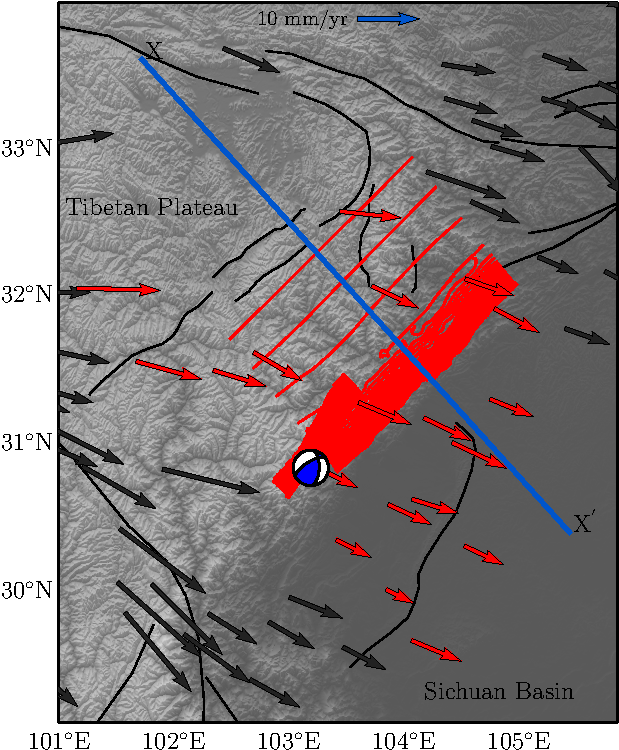
\includegraphics{figs/lms_map_all.pdf}
    \caption{Tectonic setting of the $\textrm{M}_{\textrm{w}}$ 7.9 Wenchuan earthquake and Longmen Shan rangefront. The focal mechanism is located at the epicenter of the Wenchuan earthquake and the thick red line shows the surface trace of rupture. The thin red lines show 1 km depth contours of the fault model. GPS velocity vectors (reference) are colored red if they are included in the two-dimensional models we consider. The blue line shows the two-dimensional cross-section we study. Thin black lines indicate other significant faults in the region \citep{Taylor09}.}
    \label{fig:regional_map}
\end{figure}

\section{Geodetic analysis of Longmen Shan shortening and slip deficit rates}
The geometry of the Beichaun fault and the detachment to the west have been inferred from 1) structural interpretations  \citep{Hubbard2010} (Plesch and Shaw, personal communication), 2) seismic relection observations \citep{Zhang2009, Guo2013}, and 3) geodetic modeling of co- and post-seismic deformation associated with the Wenchuan earthquake \citep{Qi2011, Fielding2013b}. The depth and dip of the detachment are similar to the best-fitting surface found by \citet{Qi2011}. The fault system geometry consists of two main segments (Figure \ref{fig:regional_map}). The range-front Beichuan fault dips steeply at ${\sim}60^{\circ}$ at its surface trace shallowing to sub-horizontal ${\sim}20$ km depth where it merges with the detachment surface. The detachment dips at ${\sim}1.5^{\circ}$ from an initial depth of 20 km and extends 110 km to the northwest to a depth of 23 km. For our interseismic shortening and slip-deficit models we use an idealized two-dimensional representation of these fault surfaces (Figure \ref{fig:regional_map}).

The inference that a 20 km deep detachment slipped, either co- or post-seismically, at distances up to 100 km from the range-front \citep{Qi2011}, necessitates including interseismic GPS velocities at a similar distance into the interior of the Tibetan Plateau (Figure \ref{fig:regional_map}). We analyze interseismic GPS velocities measured during the decade prior to the Wenchuan earthquake \citep{gan07}, in a nominally Eurasian reference frame \citep{apel06}. We exclude velocities that are near other major active structures including the Xianshuihe and Kunlun faults (Figure \ref{fig:regional_map}). 

To model both the tectonic and earthquake cycle processes contributing to these interseismic GPS data, we use a quasistatic elastic boundary element software under active development. An important feature of our tool is the inclusion of accurate surface topography in steep mountainous regions or Earth curvature in large-scale problems. Previous boundary element methods in the earth sciences \citep{Thomas1993, Maerten2014a} have been based on analytic integrations of rectangular or triangular slip surfaces \citep{Okada1992, Meade2007}. These analytic formulae normally assume an infinite half-space geometry and piecewise constant slip. Even so, they are time consuming to derive. To avoid these limitations, the basis for our boundary element formulation is numerical quadrature of the integrals in the full-space elastic Somigliana identity \citep{Cruse1969}. The difficulty in this approach is that straightforward quadrature methods (for example, Gaussian quadrature) assume a smooth integrand. For observation points on or very close to a surface, including the free surface, the integrand is singular. We resolve this problem by evaluating singular integrals as the limit of a sequence of non-singular integrals. This approach is similar to analytical limit-to-the-boundary methods \citep{Sutradhar2008} and series-expansion methods \citep{Klockner2013}. Our tests of relative error show that this quadrature-based method can match, to arbitrary precision, analytically derived half-space solutions and is free of the singularities present in those solutions. This entirely numerical boundary element method allows for complete flexibility in representing both variable surface topography and complex fault system geometeries. The steep topography of the Longmen Shan rangefront is included via the SRTM30\_PLUS digital elevation dataset \citep{Becker2009}.

Using this boundary element model, we solve for the single best-fitting shortening rate between the Tibetan Plateau and the Sichuan Basin while maintaining kinematic consistency using a two-dimensional block formulation. In the block formulation, the slip-deficit rate on the fault, $s_\mathrm{sd}$, is related to the local fault dip, $\delta$, and total convergence rate, $v_0$, by $s_\mathrm{sd}=v_0 / \cos\delta$ \citep{mccaffrey02, Meade2005}. As a result, slip-deficit rates are strictly larger than shortening rates to maintain smoothly varying horizontal surface velocities. The average interseismic slip-deficit on the fault geometry is subtracted from block motion to calculate the interseismic velocity profile \citep{savage83, Meade2005}. 

\begin{figure}[h!]
    \centering
    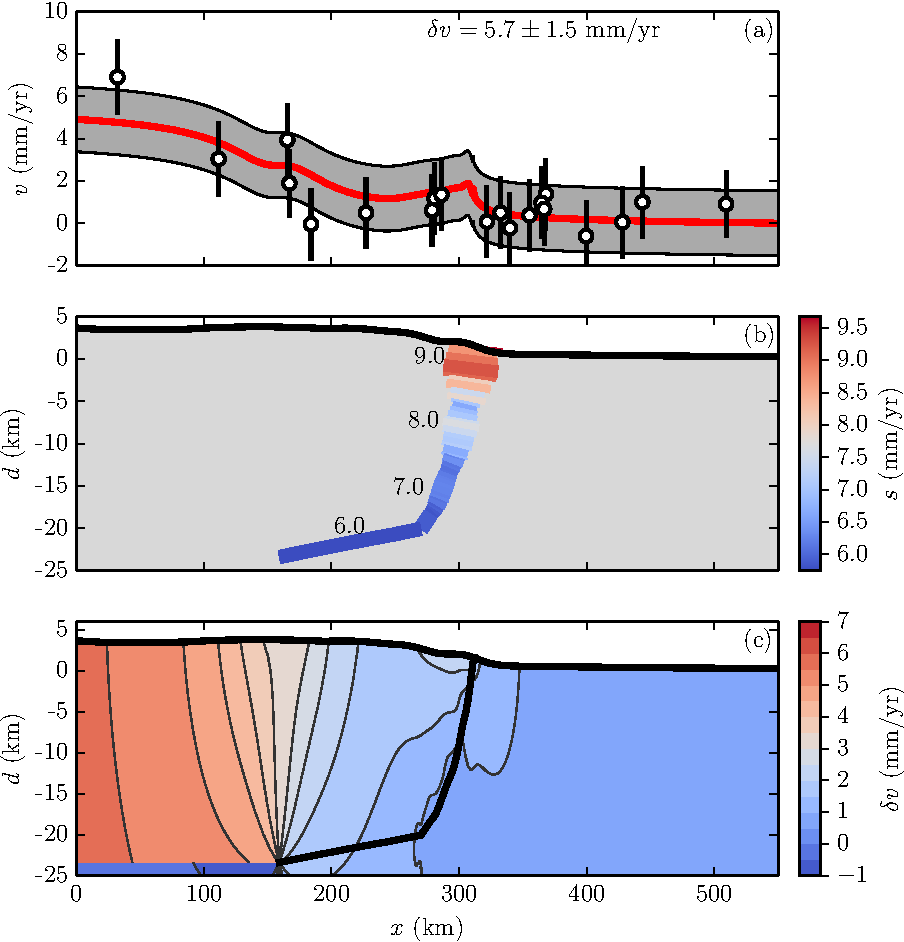
\includegraphics{figs/stack_figure_all_details.pdf}
    \caption{GPS velocities, model geometry, and inferend slip-deficit rates. a) Observed profile-parallel horizontal observed velocities are shown in black with 68\% confidence errorbars. Model-predicted velocities are shown by the red line with the surrounding gray region showing a 68\% confidence interval. b) Model geometry with colors and width along the locked fault showing predicted slip-deficit rates. Because shortening is the horizontal component of slip-deficit, increasing dips near the surface lead to larger slip-deficits. c) Predicted horizontal velocity as a function of depth. Note the steep velocity gradient and corresponding strain accumulation above the end of the detachment surface. Vertical axes are exagerated in all panels.}
    \label{fig:big_stack}
\end{figure}

The velocity gradient across the Longmen Shan rangefront is negligible (Figure \ref{fig:big_stack}a). To fit these observed near-field data, a Beichuan-only fault geometry, dipping ${\sim}60^{\circ}$ at the surface and shallowing to ${\sim}10^{\circ}$ at a maximum locking depth of 20 km would require near-zero slip-deficit rates. Such a model is inconsistent with slip during the Wenchuan earthquake on the Beichuan and Penguan faults. It is also inconsistent with co- and post-seismic slip on the detachment \citep{Qi2011, Fielding2013b}.

The inclusion of a locked detachment, however, shifts the predicted location of the steep interseismic velocity gradient far to the northwest (Figure \ref{fig:big_stack}a). When including a locked detachment, the least squares best-fit shortening rate for the Longmen Shan region is 5.7 $\pm$ 1.5 mm/yr. The spatial distribution of interseismic deformation is affected by the fault geometry and kinematic consistency constraints and represented in terms of the slip-deficit rate which ranges from ~6.0 mm/yr on the deep detachment to 9.5 mm/yr at the surface trace of the Beichuan fault (Figure \ref{fig:big_stack}b). Figure \ref{fig:big_stack}c shows the horizontal velocities as a function of depth, demonstrating that the velocity gradients derive from a locked to creeping transition at the detachment tip. The smoothing behavior of an elastic Earth prevents distinguishing between a sharp drop in slip-deficit and a gradual change over many kilometers. These results demonstrate a mechanism for a distinct interseismic strain accumulation to be most clearly manifest far from the range-front structures on which coseismic slip is greatest.

The primary uncertainty in our shortening estimate is the lack of good constraints on the detachment geometry in the hinterland. However, assuming the geometry is correct, two further forms of error are evident. First, the uncertainty in true interseismic velocities is propagated through to the estimated shortening, resulting in the gray region of uncertainty in Figure \ref{fig:big_stack}a. Further, the sparsity of observations suggests that certain observations may have undue influence on the shortening estimate. Excluding the northwest-most observation decreases the best-fit shortening to 3.9 $\pm$ 1.9 mm/yr, with a near-surface slip-deficit rate of 6.5 (give uncertainty) mm/yr on the Beichuan fault. The least squares uncertainty is increased (from 1.5 mm/yr to 1.9 mm/yr) because the northwestern portion of velocities are poorly constrained once the observation is excluded. This northwestern-most observation is adjacent to the Longriba fault, suggesting that it should not be included. However, the Longriba fault is primarily a dextral strike-slip fault \citep{Ren2013}, so it's influence should be predominantly orthogonal to the profile parallel velocities we examine here.

To further quantify the sensitivity of slip-deficit rate estimates to variability in data selection we perform a complete case resampling bootstrap shortening and slip-deficit rates are calculated for all possible subsets of the observed GPS velocities. There only $2^{20} = 1,048,576$ possible subsets of the observations (Figure \ref{fig:distribution}). We sample jointly from this distribution and the distribution of surface-area weighted fault depths. This analysis demonstrates that the majority of the slip-deficit-depth probability landscape lies at slip-deficit rates between 4 and 6 mm/yr. In the steepest, near-surface portion of the rangefront has minimum slip-deficit rates of ${\sim}$6 mm/yr, with an ${\sim}$25\% chance of slip-deficit rates above 10 mm/yr (Figure \ref{fig:distribution}). This geodetically constrained slip deficit rate can provide a mechanism for the rapid loading of the faults which exhibited 5-7 m of near-surface coseismic slip during the Wenchuan earthquake \citep{Xu2009, Shen2009b}. 

\begin{figure}[h!]
    \centering
    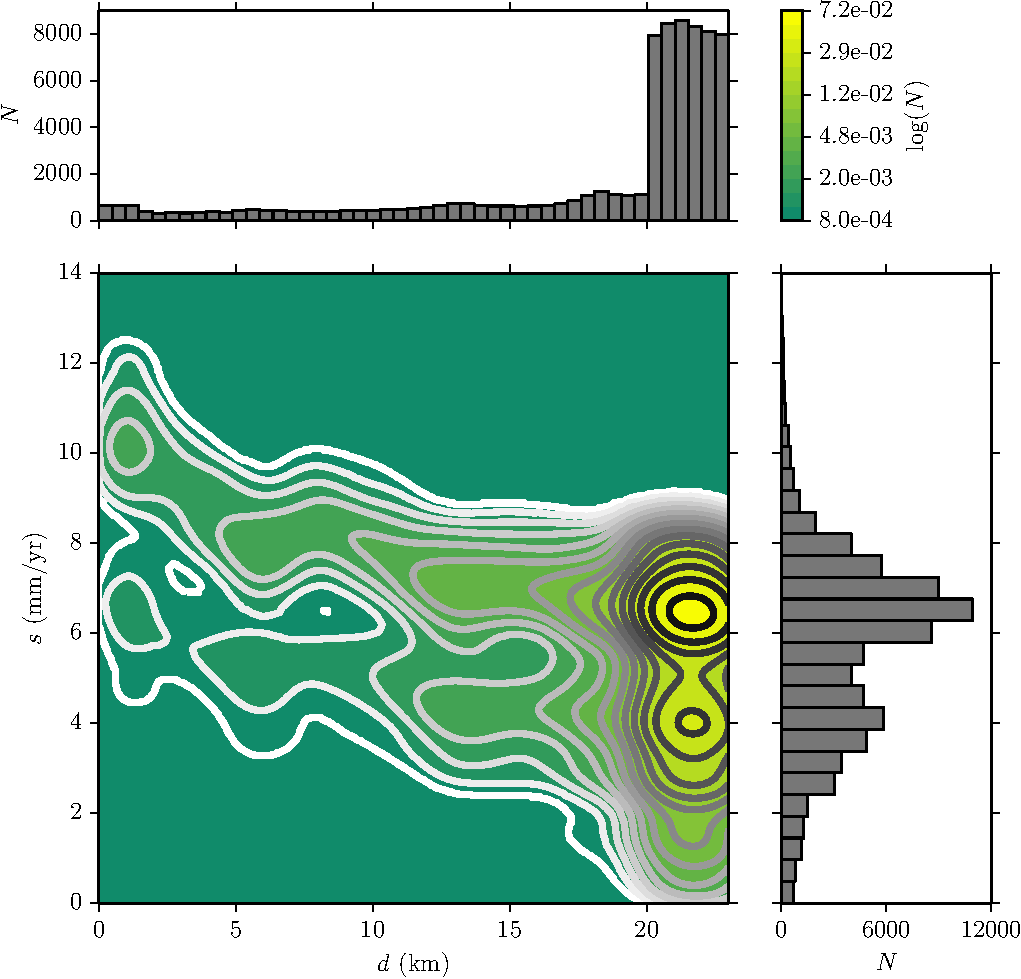
\includegraphics{figs/depth_slip_contour.pdf}
    \caption{The depth-slip-deficit probability landscape. The upper histogram is the projection of the contour plot onto a depth histogram, demonstrating that the majority of the fault surface area lies on the deep detachment. The right histogram is the projection of the contour plot onto a slip-rate histogram showing that the majority of fault surface area is slipping at rates near 6 mm/yr.}
    \label{fig:distribution}
\end{figure}

\section{Implications for the Longmen Shan earthquake cycle}
The fundamental effect of allowing a 20 km detachment to accumulate and release elastic strain through the earthquake cycle is the lack of a range-front geodetic signature despite the significant ($5-10$ mm/yr) slip-deficit rate (\ref{fig:big_stack}a). Locking on the deep detachment obscures the signal of deformation on the range-front faults. The interseismic deformation is much more broadly distributed across more than 300 kilometers. According to this model, interseismically, the eastern Tibetan Plateau moves cohesively with the Sichuan Basin, whereas coseismic slip is concentrated at the boundary between these two blocks.

Prior analyses of interseismic deformation at the Longmen Shan including the effects of dipping fault system geometry and earthquake cycle effects have been limited \citep{Loveless2011, Qi2011, Hao2014}. Of these only the three-dimensional block model of \citet{Loveless2011} is kinematically consistent \citep{minster87,mccaffrey02,Meade2005}. Compared to their estimated slip rate of 3.2 mm/yr, our estimate is $2.5 \times$ as large.  Their calculations indicate a maximum 37\% likelihood of internal block strain west of the Longmen Shan region \citep{Loveless2011}. Attributing that block-internal strain to a deep detachment instead can explain the discrepancy between the two models. Our model of far-field deformation is also consistent with a similar detachment model of leveling and GPS-based uplift rates \citep{Hao2014}. The vertical velocities they measure increase from the Longmen Shan rangefront until peaking 50 km southeast of the Longriba fault zone at approximately 3.5 mm/yr of uplift. The Longriba fault zone has the wrong slip-sense (thrusting up to the south-east, \citep{Ren2013}) to accomodate such vertical deformation. No other identified structures are nearby. 

The velocity gradient which we link to the physics of the earthquake cycle and mapped fault system geometry has been alternatively asserted to represent distributed strain across the eastern Tibetan Plateau \citep{Royden2008}. Relatedly, \citet{kirby07} study an eastward decrease in interseismic velocities across the Kunlun fault. They conclude that the decline in slip-rate must be attributed to internal deformation. Further, fast erosion and inferred uplift rates have been used to support lower crustal inflation models in the absence of shortening \citep{Kirby2003}. All of these features can be explained with slip accomodated by a wide eastern Tibetan fold-and-thrust system, a suggestion supported by the continuation of shortening north from the Longmen Shan onto the Huya \citep{kirby00} and Min Jiang faults \citep{Chen1994}. 

While we have explained the observed the broad GPS interseismic velocity gradient as a result of a locked fault geometry including a deep detachment, we have not addressed when accumulated slip-deficit on the deep detachment is released. Geodetically constrained estimates of co- and post-seismic slip shows up to 5 m of slip on a deep detachment \citep{Qi2011}. Our data analysis depends on the detachment being locked during the period of data collection from 1998 to 2004 \citep{gan07}. In addition to coseismic and short-term postseismic activity on the detachment, it is possible that intermittent aseismic slip could be an important mode of strain release. This is difficult to observationally constrain given that intersimsic GPS observations cover, at best, 6\% of a complete Longmen Shan earthquake cycle. Seismicity is approximately limited to the upper 20 km of crust in the range-front \citep{Li2010a}. Using steady-state critical taper wedge theory \citep{dahlen90}, with a internal coefficient of friction of 0.7, a cohesion of 5 MPa, and a hydrostatic fluid pressure, we find a basal friction coefficient of 0.08. This is comparable to estimates of friction on the low-angle detachment system beneath the Longmen Shan foreland \citep{Hubbard2010}, indicating a very weak fault over long time-periods. On the other hand, the surface area and shortening rate of the detachment could sustain very large earthquakes if slip is released coseismically. Specifically, if 100 km down-dip and 300 km along-strike were to slip 4 meters, similar to average slip during the Wenchuan earthquake, a $\textrm{M}_{\textrm{w}}$ 8.4 rupture would be produced.

We also quantify the effect of explicitly treating surface topography by comparing models with and without surface topography, the local minimum in velocity (Figure \ref{fig:big_stack}a) northwest of the Beichuan is identified as the main topographically-influenced feature. The effects may be more pronounced with a shallower fault dip (e.g., many subduction zones). Despite the mediocre effect (${\sim}$15\%), geodetic analyses in steep regions should consider topographic effects to avoid systematic bias. This effect may be even more pronounced for coseismic faulting where deformation is localized in regions of steep topography.

The 6-9 mm/yr slip-deficit rates estimated here can be used to provide a new kinematic constraint on earthquake recurrence intervals at the Longmen Shan (Figure \ref{fig:hazard}). Our shortening estimate suggests a recurrence interval for Wenchuan-like ruptures of approximately 600 years, with much shorter recurrence intervals for smaller events. This contrasts with the average recurrence of ~2000 years inferred from paleoseismic field investigations for the Beichuan fault \citep{Ran2010}. The 6-9 mm/yr slip-deficit rate estimated here would imply $\textrm{M}_{\textrm{w}}$ 9.0 ruptures for that recurrence interval, which would seemingly require an along strike rupture equal to or greater than the ${\sim}300$ km along strike length of the Longmen Shan. However, our slip-deficit estimate could include the effects of other imbricated structures. As a result our estimate is a system-wide estimate while paleoseismic estimates have focused on the analysis of individual thrust faults. 


The earthquake recurrence intervals calculated above may be considered a lower bound. First, coseismic, interseismic, and geologic slip estimates include a significant component of strike-slip motion \citep{Shen2009a, Qi2011, Densmore2007, Meade2007, Loveless2011}, while we consider an idealized case of fault normal motion only. Second, our two-dimensional model assumes plane strain conditions which will result in under-estimates of the shortening required to produce far-field velocities. This is because the plane strain simplification is equivalent to assuming the fault geometry extends infinitely far along strike. Third, the modeled thrust is the steeply dipping Beichuan fault. The foreland Range Front thrust or the shallow detachment beneath Chengdu dip more shallowly \citep{Hubbard2010}, producing a greater total moment deficit. Finally, the slip-deficit rate estimates may be low due to being estimated late in the earthquake cycle (i.e., in the decade prior to the Wenchuan earthquake) when viscoelastic effects may further contribute to a low near fault trace velocity gradient \citep{savage00}.

\begin{figure}[h!]
    \centering
    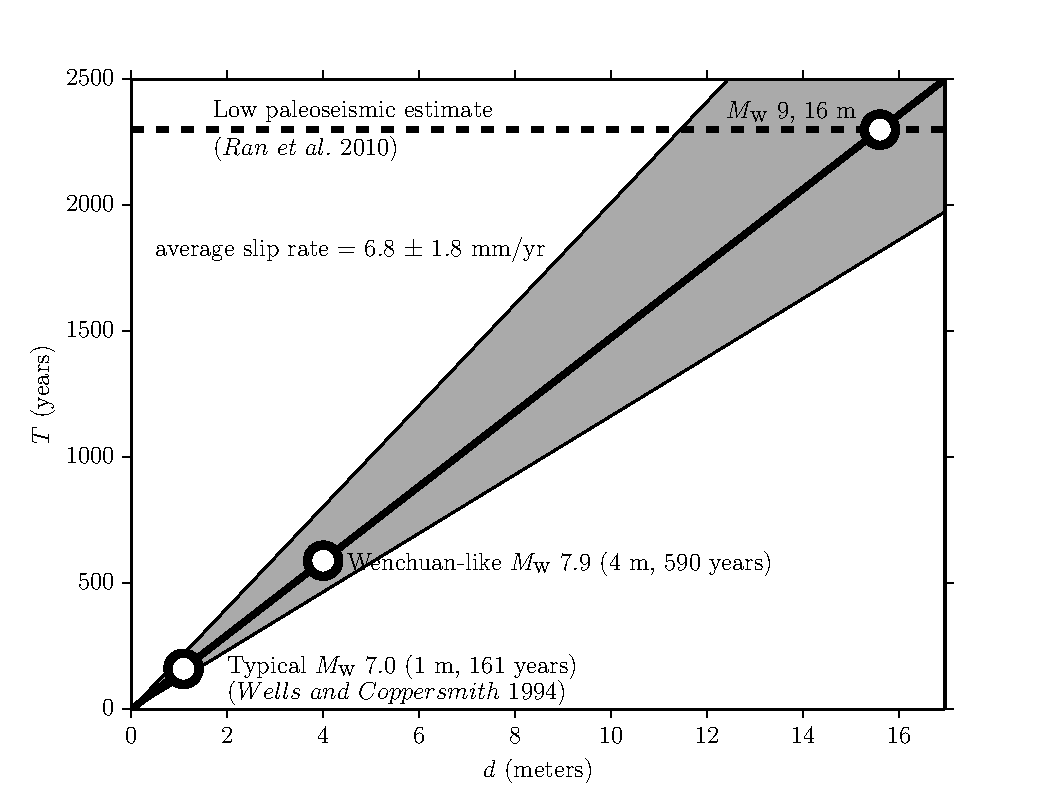
\includegraphics{figs/hazard_all_details.pdf}
    \caption{Earthquake recurrence intervals as a function of coseismic slip, assuming the best-fit slip rate for the Beichuan fault. The gray region indicates the uncertainty implied by the error in our shortening estimate. The discrepancy between the Wenchuan-like recurrence and the paleoseismic estimate may be due to the presence of multiple active faults in the range-front. (BJM note: Fixe the Ms in the figure so that they are not italicized and consistent with other in the text)}
    \label{fig:hazard}
\end{figure}

\section{Conclusion}
Previous inferences of near-zero interseismic shortening estimates at the Longmen Shan have been difficult to reconcile with the large-moment of the Wenchuan earthquake, very steep topography, structural interpretations indicating fold-and-thrust geometry, and fast erosion rates. We offer a possible resolution to this conflict by including earthquake cycle effects associated with interseismic locking on the Beichuan fault and a 20 km deep detachment to the west. Our revised interseismic shortening rate is 5.7 $\pm$ 1.5 mm/yr with on-fault slip-deficit rates up to 9.5 mm/yr near the surface where the Beichuan fault is most steeply dipping. The model demonstrates that interseismic strain accumulation may be spatially disjoint from coseismic strain release, emphasizing that accurate fault system geometries are critical in the analysis of geodetic data. The boundary element model presented here unifies geodetic models of coseismic, postseismic and interseismic crustal deformation across the greater Longmen Shan region and suggests that, with current loading rates, Wenchuan-like earthquakes may occur as frequently as every 600 years.

\bibliographystyle{Jcks}
\bibliography{biblio,library}
\end{document}
